\chapter{Design}

\section{Conceptual Model}

\subsection{State Diagram}
\begin{figure}[ht]
\centering
\empuse{erdiag}
\caption{Entity Relationship Diagram}
\end{figure}
\FloatBarrier

\subsection{Activity Diagrams}

\begin{figure}[ht]
\centering
\empuse{activityR1}
\caption{Activity Diagram: Creating a project.}
\end{figure}


\begin{figure}[ht]
\centering
\empuse{activityR2}
\caption{Activity Diagram: Creating a team.}
\end{figure}


\begin{figure}[ht]
\centering
\empuse{activityR4}
\caption{Activity Diagram: Assigning tasks.}
\end{figure}
\FloatBarrier

\subsection{Mockups}

\begin{figure}[ht]
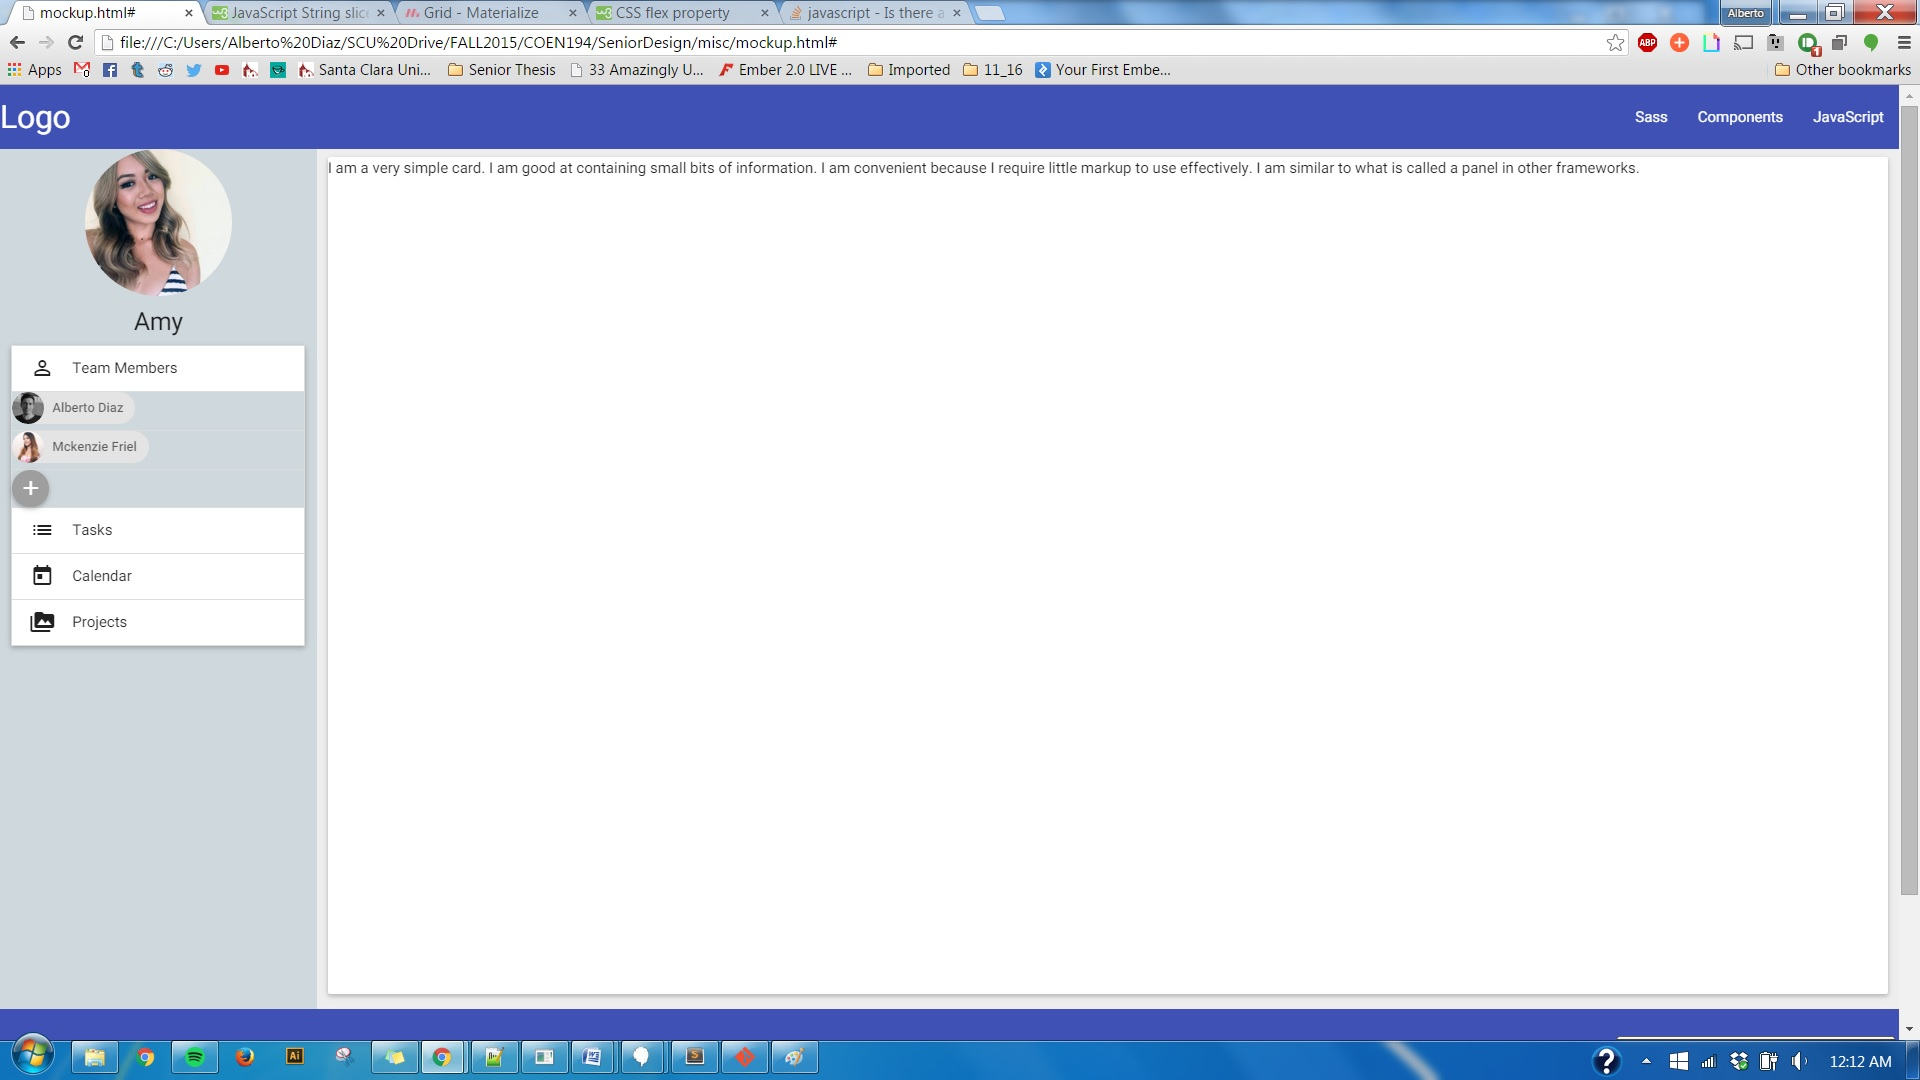
\includegraphics[width=\textwidth]{mockup.jpg}
\caption{A mockup of our system concept.}
\end{figure}
\FloatBarrier

\section{Use Cases}

\begin{figure}[ht]
\centering
\empuse{usecasediag}
\caption{Use Case Diagram}
\end{figure}

\begin{figure}[ht]
\begin{usecase}

\addtitle{Use Case 1}{Create Project} 

\addfield{Goal:}{Initialize project objectives, tasks, and deadlines}

\addfield{Actor:}{User}

\addfield{Preconditions:}{Account is set up}
%when multiple
%\additemizedfield{Preconditions:}{} 

\addfield{Postconditions:}{Project is initialized}
%when multiple
%\additemizedfield{Preconditions:}{}

%Main Success Scenario: A typical, unconditional happy path scenario of success.
\addscenario{Steps:}{
  \item Name the project
  \item Define project goals and deadlines
  \item Add people to the project
  \item Save the project
}

%Extensions: Alternate scenarios of success or failure.
\addscenario{Exceptions:}{
  \item[A.] Invalid login data:
    \begin{enumerate}
    \item[1.] System shows failure message
    \item[2.] User returns to step 1
    \end{enumerate}
  \item[B.] Invalid subsriber data:
    \begin{enumerate}
    \item[1.] System shows failure message
    \item[2.] User returns to step 2 and corrects the errors
    \end{enumerate}
}
\end{usecase}
\end{figure}
\begin{figure}[ht]
\begin{usecase}

\addtitle{Use Case 1}{Template test} 

\addfield{Goal:}{System-wide}

\addfield{Actor:}{End-User}

\addfield{Preconditions:}{}
%when multiple
%\additemizedfield{Preconditions:}{} 

\addfield{Postconditions:}{}
%when multiple
%\additemizedfield{Preconditions:}{}

%Main Success Scenario: A typical, unconditional happy path scenario of success.
\addscenario{Steps:}{
  \item The first action
  \item The second action
}

%Extensions: Alternate scenarios of success or failure.
\addscenario{Exceptions:}{
  \item[2.a] Invalid login data:
    \begin{enumerate}
    \item[1.] System shows failure message
    \item[2.] User returns to step 1
    \end{enumerate}
  \item[5.a] Invalid subsriber data:
    \begin{enumerate}
    \item[1.] System shows failure message
    \item[2.] User returns to step 2 and corrects the errors
    \end{enumerate}
}
\end{usecase}
\end{figure}
\begin{figure}[ht]
\begin{usecase}

\addtitle{Use Case 1}{Template test} 

\addfield{Goal:}{System-wide}

\addfield{Actor:}{End-User}

\addfield{Preconditions:}{}
%when multiple
%\additemizedfield{Preconditions:}{} 

\addfield{Postconditions:}{}
%when multiple
%\additemizedfield{Preconditions:}{}

%Main Success Scenario: A typical, unconditional happy path scenario of success.
\addscenario{Steps:}{
  \item The first action
  \item The second action
}

%Extensions: Alternate scenarios of success or failure.
\addscenario{Exceptions:}{
  \item[2.a] Invalid login data:
    \begin{enumerate}
    \item[1.] System shows failure message
    \item[2.] User returns to step 1
    \end{enumerate}
  \item[5.a] Invalid subsriber data:
    \begin{enumerate}
    \item[1.] System shows failure message
    \item[2.] User returns to step 2 and corrects the errors
    \end{enumerate}
}
\end{usecase}
\end{figure}
\FloatBarrier

\section{Architectural Design}
\begin{figure}[ht]
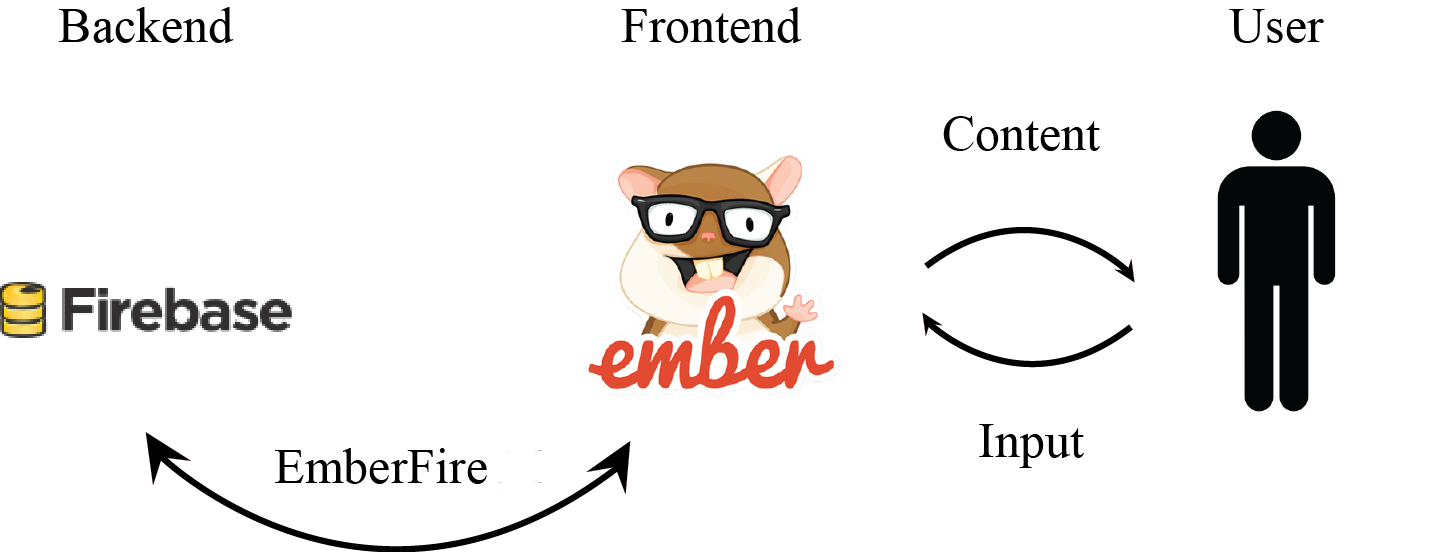
\includegraphics[width=\textwidth]{archDiag.png}
\caption{Diagram describing the technology stack for our application.}
\end{figure}
\FloatBarrier

\section{Technologies Used}
In this section, we describe the technologies we chose to develop our application and the features they provide for us.
\begin{enumerate}
\item HTML5 \par The latest version of the standard web markup language
\item JS \par A high-level, untyped, and interpreted programming  language supported by all modern web browser
\item CSS3 \par A stylesheet language used to describe the presentation of HTML documents
\item Ember.js \par A front-end javascript framework based on the model-view-controller (MVC) model and applies programming conventions to build scalable applications
\item  Firebase \par A backend-as-a-service that provides client-side APIs, and services such as databases, web hosting, and authentication.
\end{enumerate}

\section{Design Rationale}
In this section, we describe why we chose these technologies and the advantages and disadvantages associated with each of those technologies. 
\begin{enumerate}
\item HTML5/CSS3 /JS \par The latest version of the standard web markup language
	\begin{enumerate}
	
	\end{enumerate}
\item Ember.js \par A front-end javascript framework based on the model-view-controller (MVC) model and applies programming conventions to build scalable applications
\item  Firebase \par A backend-as-a-service that provides client-side APIs, and services such as databases, web hosting, and authentication.
\end{enumerate}